\chapter{研究问题简述}
在本章节中,我们将对图像修复问题进行深入的探讨,并明确本文研究的具体问题。首先,通过梳理已有文献,我们回顾了图像去噪问题的研究背景,对其发展历程和现状进行了概述。在此基础上,我们进一步定义了图像修复问题中的关键概念和符号,为后续的研究奠定了理论基础。通过本章节的阐述,我们希望能够为读者提供一个清晰的图像修复问题概述,并引出本文所要解决的具体问题。
\section{背景回顾}
本文的主要研究问题为对目标图像进行去噪处理,得到相应去噪前的可能图像的生成。首先回顾传统生成模型的适用条件与背景。传统的扩散模型,如\cite{song_2,DDPM,DDIM}中的扩散模型,均用于实现从纯噪声图片生成原图像分布。其中最关键的步骤为Score-matching, 即为通过参数拟合学习得到真实的对数密度函数的梯度。即假设原定未知目标分布为$X_0\sim p(X_0)$, 通过构造扩散过程得到随机过程$X_{0:T}$使得$p(X_{T})\sim \mathcal{N}(0,I)$(或者使得分布趋近于标准正态分布即可)。 Score-matching即为,在选取较大的$T$的情况下,学到$\nabla_{X_t}\log (p(X_t))$的值,记该函数为Score-function。     

在\cite{song_2}中主要采用解逆向随机微分方程来获得对目标未知分布的一个采样。问题设定主要如下:   

目标未知分布为$x\sim p(x_0)$,其中$x\in \mathbb{R}^n$, 通过构造扩散过程
\begin{equation}
    dx = f(x,t)dt + g(t)dW_t,
    \label{diffusion equation SDE 1}
\end{equation}
其中$W_t$为标准 $d$维 布朗运动,以$x_0$为初始随机变量,实际通过欧拉法离散化生成$x_{i/T}$, $i=1,\cdots, T$, 最后采样得到$x_1$。通过设计特定形式的随机微分方程(\ref{diffusion equation SDE 1}),可以使得最终随机变量$x_1$的概率分布为形式较为简单的概率分布 (例如为标准高斯分布)。以下定义两种通常使用的随机微分方程来对初始输入进行扩散, 
\begin{definition}[VP-SDE, 方差收缩随机微分方程]
\label{VP-SDE def}
    我们定义如下随机微分方程为VP-SDE,即Variance Preserving SDE。对于随机过程$\{x_t\}_{t\in [0,1]}$, 满足随机微分方程
    \begin{equation}
   \mathrm{d} \mathbf{x}=-\frac{1}{2} \beta(t) \cdot \mathbf{x} \mathrm{d} t+\sqrt{\beta(t)} \mathrm{d} \mathbf{w}, \label{VP-SDE equation} 
    \end{equation}
    该随机过程满足如果初始输入$x_0$为标准化后\footnote{满足数学期望为0,方差为1的随机变量}的随机变量,则对于任意$t\in [0,1]$,我们都有
    \begin{equation}
        \mathbb{E}\left[x_t\right]=0, \operatorname{Var}\left(x_t\right)=1 .
        \label{Normalizing condition}
    \end{equation}
    该结论见如下证明。
\end{definition}
以下证明在\ref{VP-SDE def}中对标准化输入的性质的证明,
\begin{proof}
    利用伊藤公式,我们引入如下记号,我们定义$p(t) = \mathbb{E}\left[x_t\right],q(t) = \mathbb{E}\left[x_t^2\right]$. 在已知式\ref{VP-SDE equation}的条件下,我们有
    \begin{equation}
        dp(t) = -\frac{\beta(t)}{2}p(t),
    \end{equation}
    因此可以得到$p(t) = p(0)e^{-\int_{0}^t \beta(s)/2\mathbf{d}t} = 0 $, 对于任意$t\in [0,1]$, 此处用到了初始条件$\mathbb{E}\left[x_0\right]=0=p(0)$, 因此$\operatorname{Var}\left(x_t\right)=\mathbb{E}\left[x_t^2\right]$。同样利用式(\ref{VP-SDE equation})和伊藤公式,我们有
    \begin{equation}
        dX_t^2 = \left(-\beta(t)x_t^2 + \beta(t)\right)dt + 2x_t \sqrt{\beta(t)} \mathrm{d} \mathbf{w},
    \end{equation}
    对等式两边同时取数学期望可得
    \begin{equation}
        dq(t) = -\beta(t) \left(q(t)-1\right)\mathbf{d}t,
    \end{equation}
    因此我们有$q(t) = 1 + \left(q(0)-1\right)e^{-\int_{0}^t \beta(s)\mathbf{d}s}= 1$, 此处用到了初始条件式(\ref{Normalizing condition})中的$q(0)=1$。
\end{proof}

同时我们引入另一类常见在扩散模型中使用的随机微分方程,即方差爆炸随机微分方程,见如下定义。
\begin{definition}[VE-SDE, 方差爆炸随机微分方程]我们定义以下随机微分方程为VE-SDE,即Variance Exploding SDE。对于随机过程$\{x_t\}_{t\in [0,1]}$, 满足随机微分方程
    \begin{equation}
        dx_t = \sqrt{\frac{d\left[\sigma^2(t)\right]}{dt}}\mathbf{d}\mathbf{w}, \label{VE-SDE}
    \end{equation}
    其中$\sigma(t)$为$[0,\infty]\xrightarrow{}\mathbb{R}^+$的严格递增光滑函数满足$\sigma(0)=0$,当$t\to \infty$,我们有 $\sigma(t)\xrightarrow{}\infty$。
    对于满足随机微分方程(\ref{VE-SDE})的随机过程$\{x_t\}_{t\geq 0}$,随着$t\to \infty$, 有$\operatorname{Var}(x_t)\xrightarrow{}\infty$,因此称其为方差爆炸方程。 
\end{definition}

例如我们可以不断对初始输入$x_0$不断增加白噪声(进行加权组合),最终使得其分布不断趋紧与白噪声的分布(例如VP-SDE和VE-SDE中的情形)。 为了还原采样得到初始图像的分布,我们只需要从白噪声开始进行逆向采样,只要知道逆向随机微分方程的信息,即可以进行还原操作。 首先我们需要引入逆向随机微分方程的结论,见如下定理。

\begin{theorem}[逆向随机微分方程]
在已知(\ref{diffusion equation SDE 1}) 的形式的情形下,存在以$x_1$为初始值的逆向随机微分方程
\begin{equation}
     dx_t= \left(f(x,t)-g^2(t)\nabla_{x_t}\log(q_t(x_t))\right)dt + g(t)d\Tilde{w}_t,
    \label{reverse diffusion equation SDE 1}
\end{equation}
其中$\{\Tilde{w}_t\}_{t\in [0,1]}$也为标准布朗运动,我们定义$s(t,x_t) = \nabla_{x_t}\log(q_t(x_t))$ 为打分函数(score function)。
\end{theorem}
    此处我们直接引用部分\cite{Anderson1982ReversetimeDE}中的结论, 其中逆向随机微分方程(\ref{reverse diffusion equation SDE 1})中的标准布朗运动$\{\Tilde{W}_t\}_{t\geq 0}$满足如下随机微分方程
    \begin{equation}
     \mathrm{d} \Tilde{w}_t^k=\mathrm{d} w_t^k+\frac{1}{p\left(x_t, t\right)} \sum_j \frac{\partial}{\partial x_t^j}\left[p\left(x_t, t\right) g^{j k}\left(t\right)\right] \mathrm{d} t,
        \label{Tilde W SDE equation}
    \end{equation}
其中$\Tilde{w}_t^k$, $w_t^k$ 分别表示$\Tilde{w}_t$ 和 $w_t$ 的第$k$ 个分量, $p(x_t,t)$表示在扩散过程$t$时刻的随机变量$x_t$所满足的密度函数 (我们假设所有随机变量均为连续分布的随机变量因此存在良好定义的密度函数), $g^{jk}$表示$g(t)$ (形状为$n\times d$的矩阵函数中第一$j$行第$k$列的元素)。 

因此只需要得到打分函数(Score function)的信息,即可从$x_1$开始逆向利用欧拉法进行离散化取样,当步长$T$足够大的时候,则离散化间距$1/T$足够小, 根据 
\cite{detemple}中对于Monte Carlo Estimator的渐进性质的分析,在使用Euler 法进行离散化取样的时候可以以$1/\sqrt{T}$的收敛速度趋近真实随机变量的分布;当采用Doss Transformation使得随机变量的随机微分方程的Diffusion 项为非随机量的时候,则可以以$1/T$的速率分布上收敛至真实分布。考虑到(\ref{diffusion equation SDE 1})的形式,通常取$T=1000$量级的步长已经可以有较好的逼近效果。      

由于在(\ref{reverse diffusion equation SDE 1})中唯一的位置量即为目标函数Score function $\nabla_{x_t}\log(q_t(x_t))$, 可以用一个和时间和随机变量本身相关的函数$S_{\theta}(t,x)$ 来逼近,其中$\theta$为该函数的参数化。具体优化参数的方式即为
\begin{equation}
{\theta}^*=\underset{{\theta}}{\arg \min } \mathbb{E}_t\left\{\lambda(t) \mathbb{E}_{\mathbf{x}(0)} \mathbb{E}_{\mathbf{x}(t) \mid \mathbf{x}(0)}\left[\left\|\mathbf{s}_{{\theta}}(\mathbf{x}(t), t)-\nabla_{\mathbf{x}(t)} \log p_{0 t}(\mathbf{x}(t) \mid \mathbf{x}(0))\right\|_2^2\right]\right\},
\label{score matching}
\end{equation}
其中$\lambda(t)$, $t\in [0,1]$为设置的权重函数,旨在使得优化得到的权重函数不仅仅在优化某些特定时刻的误差。优化得到最佳的打分函数Score function 的优化过程 (\ref{score matching}) 即为Score matching。    


根据\cite{score_based_SDE}中通过解逆向随机微分方程的想法,可以通过设计不同的随机微分方程形式来得到不同的采样方式,以及可以设计不同的正向采样和逆向采样算法,可以让生成方式为Markovian的也可以为Non-Markovian的。在\cite{DDPM}中设计了一种特定的随机微分方程来进行采样生成,方程满足如下形式。
\begin{equation}
    dz = -\left(\beta(t)/2\right)z dt + \sqrt{\beta(t)}dW_t,
    \label{DDPM Equation}
\end{equation}
在进行离散化取样生成正向传播链的时候,可以表达为目标分布为$x_0$,从$x_0$开始正向传播生成$x_{1:T}$, 满足条件概率分布为
\begin{align}
    q\left(x_{1: T} \mid x_0\right)&=\prod_{t=1}^T q\left(x_t \mid x_{t-1}\right),\\
        q\left(x_t \mid x_{t-1}\right)&=\mathcal{N}\left(\sqrt{1-\beta_t} x_{t-1}, \beta_t I\right),
        \end{align}
        \begin{equation}
            q\left(x_t \mid x_0\right)=\mathcal{N}\left(\sqrt{\bar{\alpha}_t} x_0,\left(1-\overline{\alpha_t}\right) I\right) \text { 其中 } \alpha_t=\left(1-\beta_t\right) \text { 以及 } \bar{\alpha}_t=\prod_t \alpha_t,
            \label{posterior of xt}
            \end{equation}
    正向传播的后验分布同样可以被给出:
    \begin{equation}
        q\left(x_{t-1} \mid x_t, x_0\right)=\mathcal{N}\left(\tilde{\mu}_t\left(x_t, x_0\right), \tilde{\beta}_t\right),
        \label{posterior xt 2}
        \end{equation}
        \begin{equation}
            \text {     其中 } \tilde{\mu}_t\left(x_t, x_0\right)=\frac{\sqrt{\bar{\alpha}_{t-1}} \beta_t}{1-\bar{\alpha}_t} x_0+\frac{\sqrt{\alpha_t}\left(1-\bar{\alpha}_{t-1}\right)}{1-\bar{\alpha}_t} x_t,
            \end{equation}
            \begin{equation}
                \text { 以及 } \quad \tilde{\beta}_t=\frac{1-\bar{\alpha}_{t-1}}{1-\bar{\alpha}_t} \beta_t.
                \end{equation}
该正向过程实际上对应的随机微分方程即为
\begin{equation}
    dz = -\frac{g^2(t)}{2}\cdot  z dt + g(t)dw,
\end{equation}
$x_{0:T}$的联合分布$p_{\theta}(x_{0:T})$被称为逆向过程,并且它被定义为一个Markov过程,该过程的转移分布可以从末端$p(x_T)= \mathcal{N}(x_T;0,I) $开始。由此可以写出逆向过程的联合分布函数的表达式
\begin{equation}
    p_{\theta}(x_{0:T}) := p(x_T)\prod_{t=1}^{T}p_{\theta}(x_{t-1}|x_t), p_{\theta}(x_{t-1}|x_t) :=\mathcal{N}(x_{t-1};\mu_{\theta}(x_t,t),\Sigma_{\theta}(x_t,t)).  
\end{equation}

以上为正向Markov过程所满足的条件概率分布性质,在随机优化问题中为了优化参数需要对逆向传播过程进行建模。
逆向传播过程同样可以被参数化,此处使用高斯转移分布来进行此一阶Markov逆向传播过程,满足如下表达式:
\begin{align}
    p\left(x_{0: T}\right)&=p\left(x_T\right) \prod_{t=1}^T p_\theta\left(x_{t-1} \mid x_t\right),\\
        p_\theta\left(x_{t-1} \mid x_t\right)&=\mathcal{N}\left(\mu_\theta\left(x_t, t\right), \Sigma_\theta\left(x_t, t\right)\right),
        \end{align}
        % \begin{figure}[H]
        %     \centering
        %     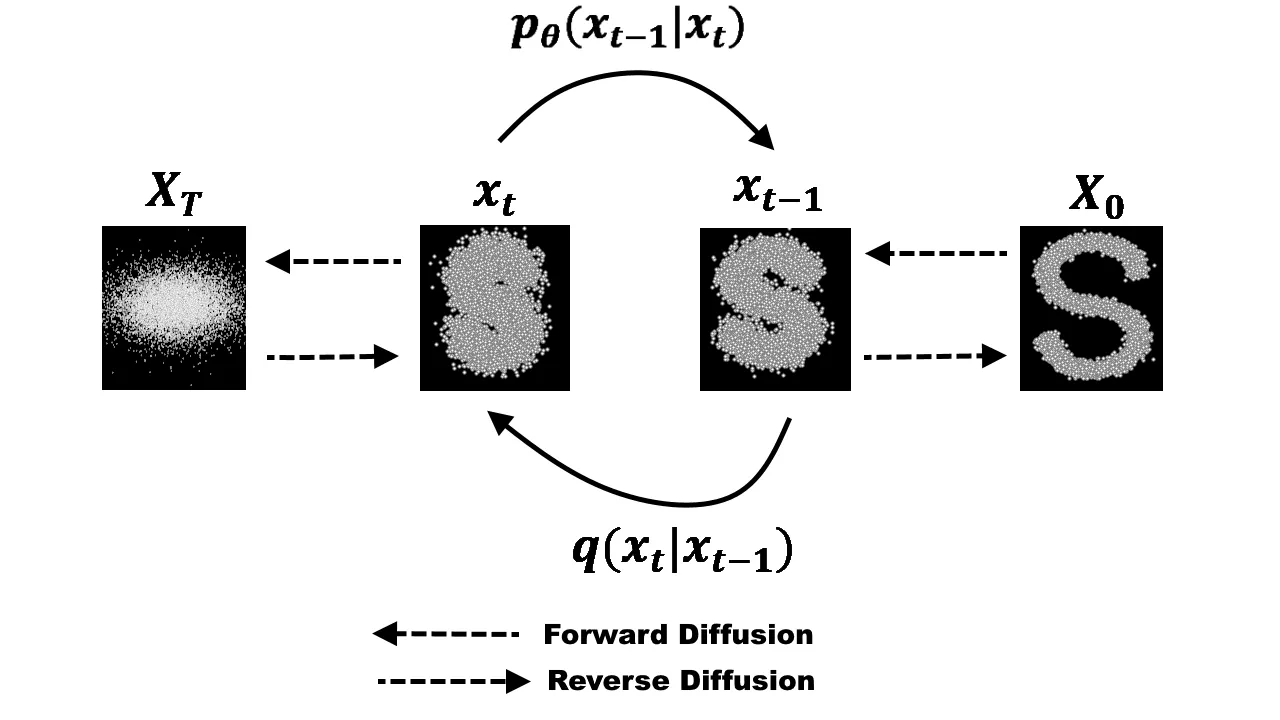
\includegraphics[scale = 0.2]{ThuThesis_ Tsinghua University Thesis LaTeX Template/Picture/Diffusion.png}
        %     \caption{扩散模型图例}
        %     \label{Diffusion}
        % \end{figure}
选取足够大的$T$值与合适的递减序列$\{\beta_t\}_{t\geq 1}$, 条件概率分布$q(x_{T}|x_0)$可以足够接近标准高斯分布。
整个概率系统可以通过变分推断来进行端到端的训练,从而优化参数。
在该模型下,同样采用极大似然估计的方式来进行参数优化,此处采用最大化对数似然函数的相反数的上界来进行优化,即
\begin{equation}
    \mathbb{E}\left[-\log p_\theta\left(\mathbf{x}_0\right)\right] \leq \mathbb{E}_q\left[-\log \frac{p_\theta\left(\mathbf{x}_{0: T}\right)}{q\left(\mathbf{x}_{1: T} \mid \mathbf{x}_0\right)}\right]=\mathbb{E}_q\left[-\log p\left(\mathbf{x}_T\right)-\sum_{t \geq 1} \log \frac{p_\theta\left(\mathbf{x}_{t-1} \mid \mathbf{x}_t\right)}{q\left(\mathbf{x}_t \mid \mathbf{x}_{t-1}\right)}\right],
    \label{DDPM objective 1}
\end{equation}
从随机优化方法的角度去考虑,可以将式(\ref{DDPM objective 1})重新写为
\begin{equation}
\mathbb{E}_q[\underbrace{\mathcal{D}_{K L}\left(q\left(x_T \mid x_0\right) \| p\left(x_T\right)\right)}_{L_T}+\sum_{t>1} \underbrace{\mathcal{D}_{K L}\left(q\left(x_{t-1} \mid x_t, x_0\right) \| p_\theta\left(x_{t-1} \mid x_t\right)\right)}_{L_{t-1}}-\underbrace{\log p_\theta\left(x_0 \mid x_1\right)}_{L_0}],
    \end{equation}
以上为DDPM的数学原理,以下将具体讨论DDPM在实际优化过程中的参数设计与模型细节。以上已经将$L$分解成$L_T,L_{t-1},L_0$三大部分,由于后验分布$q$没有任何参数,因此$L_T$可以直接忽略(和$\theta$取值近似无关)。
在\cite{DDPM}中直接假设$\Sigma_{\theta}(x_t,t)=\sigma_t^2 I$,方便简化计算过程(避免矩阵求逆运算操作)。其次,为了表示$\mu_{\theta}(x_t,t)$,由于$p_{\theta}(x_{t-1}|x_t):= \mathcal{N}(x_{t-1};\mu_{\theta}(x_t,t),\sigma_t^2I)$,我们可以将$L_{t-1}$写为
\begin{equation}
    L_{t-1}=\mathbb{E}_q\left[\frac{1}{2 \sigma_t^2}\left\|\tilde{{\mu}}_t\left(\mathbf{x}_t, \mathbf{x}_0\right)-{\mu}_\theta\left(\mathbf{x}_t, t\right)\right\|^2\right]+C,
    \label{Lt representation}
\end{equation}
其中$C$为一个和$\theta$无关的常数,在优化过程中可以被忽略。利用式(\ref{posterior of xt})可以进一步简化式(\ref{Lt representation}) 将$x_t$表示为$\mathbf{x}_t\left(\mathbf{x}_0, {\epsilon}\right)=\sqrt{\bar{\alpha}_t} \mathbf{x}_0+\sqrt{1-\bar{\alpha}_t} {\epsilon} \text { for } {\epsilon} \sim \mathcal{N}(\mathbf{0}, \mathbf{I}) $, 以及利用式(\ref{posterior xt 2})可以得到
\begin{align}
    L_{t-1}-C&=\mathbb{E}_{\mathbf{x}_0, {\epsilon}}\left[\frac{1}{2 \sigma_t^2}\left\|\tilde{{\mu}}_t\left(\mathbf{x}_t\left(\mathbf{x}_0, {\epsilon}\right), \frac{1}{\sqrt{\bar{\alpha}_t}}\left(\mathbf{x}_t\left(\mathbf{x}_0, {\epsilon}\right)-\sqrt{1-\bar{\alpha}_t} {\epsilon}\right)\right)-{\mu}_\theta\left(\mathbf{x}_t\left(\mathbf{x}_0, {\epsilon}\right), t\right)\right\|^2\right]\\
&=\mathbb{E}_{\mathbf{x}_0, {\epsilon}}\left[\frac{1}{2 \sigma_t^2}\left\|\frac{1}{\sqrt{\alpha_t}}\left(\mathbf{x}_t\left(\mathbf{x}_0, {\epsilon}\right)-\frac{\beta_t}{\sqrt{1-\bar{\alpha}_t}} {\epsilon}\right)-{\mu}_\theta\left(\mathbf{x}_t\left(\mathbf{x}_0, {\epsilon}\right), t\right)\right\|^2\right],
\end{align}
经过\cite{DDPM,score_based_SDE}中的计算化简,\ref{DDPM objective 1}实际上可以化简为
\begin{equation}
    \mathbb{E}_{t\sim \mathcal{U}(0,1),\epsilon\sim \mathcal{N}(0,I)}\left[\|\epsilon - \epsilon^{\theta}(x_t,t)\|^2\right],
    \end{equation}
而此时的打分函数满足$s^{\theta}(x_t,t) =- \frac{1}{\sqrt{\Bar{\beta}_t}}\epsilon^{\theta}(x_t,t)$,取 $\mu^{\theta}(x_t,t) = \frac{1}{\sqrt{\Bar{\alpha}_t}}\left(x_t- \sqrt{\Bar{\beta}_t}\epsilon^{\theta}(x_t,t)\right)$。 以上为DDPM主要的实现原理与优化过程。

在当下利用Diffusion Model实现图像去噪,图像修损任务中的研究中,主要采用DDPM模型中的随机微分方程进行向前扩散,以及采用和Langevin dynamic 中进行Score matching的方法进行混合使用提升收敛速率。但是实质并没有充分利用图像加噪和去噪随机变量之间的条件分布,本质上是在实现更高效率的生成式模型进行图像还原。下面进行前向加噪模型的一般形式阐述。
\section{图像修复任务}
下面进行图像修复任务的阐述,图像修复任务总体可以表述为,在前向加噪模型下,通过输入初始纯净图像$x$得到损坏图像$y$。

已知损坏图像$y$以及原始图像$x$的分布$x\sim p(x)$, 目标通过从损坏图像$y$处理还原采样得到$x^{\prime}$使得
\begin{itemize}
    \item $x^{\prime}\sim p^{\prime}(x)$, 使得后验分布$p^{\prime}(x\mid y)$ 与 $p(x\mid y)$较为接近。 
    \item  采样得到的修复图像$x^{\prime}$与原始图像$x$较为接近。 
\end{itemize}
前向加噪模型可以总体以如下形式表达:
\begin{equation}
y=\mathcal{H}\left(x_0\right)+{n}, \quad y, {n} \in \mathbb{R}^n, x \in \mathbb{R}^d,
\label{Forward model}
\end{equation}
其中$x_0$为原始分布,即为初始图像采样样本,$y$为加过噪声处理后的图像,$\mathcal{H}$为加噪算符,而$n$表示随机噪声。首先仅考虑$n$为高斯噪声的情况,即$n\sim \mathcal{N}(0,\sigma^2 I_n)$。即$y$服从条件概率分布,$y\sim \mathcal{N}(\mathcal{H}(x_0)\mid \sigma^2 I_n)$。
进一步简化问题,以及考虑实际应用中的下游任务主要集中于降噪,图像修复,去模糊化处理,超分辨率化以及等情形,在此处可假设$\mathcal{H}(\cdot)$为线性变换(线性变换可以适用于图像平移,旋转,图像部分缺损等实际应用场景),对于较为复杂的加噪模型可以在未来的工作中用泛化能力更强的模型进行去噪处理。      
\begin{definition}[图像去噪]
在加噪模型(\ref{Forward model})下,对于加噪后的图像$y$而言存在非唯一的原像。在已知去噪前图像分布数据集$p(x)$的分布和加噪图像后验分布$p(y\mid x)$的条件下,目标是得到$p(x)$内的一个子分布使得最大化后验分布$p(x\mid y)$,即采样得到原图像分布内最有可能经过加噪处理得到目标加噪图片的图像集合的分布。
\end{definition}

在图像去噪任务中,主要目标可以阐释为,在已知加噪后的图像$y$的情形下,还原得到最契合去噪前原始图像的图像分布$x\sim p(x)$,即找到最合适的随机分布$x\sim p_{\theta}(x)$,使得
\begin{equation}
 \theta^{* }= \arg\min_{\theta\in \Theta}\operatorname{KL}(q(x_0,\cdots, x_T\mid y)||p_{\theta}(x_0,\cdots,x_T\mid y)), 
\end{equation}
根据\cite{score_based_SDE}中的结论, 此时的打分函数可以变为$s(t,x_t) = \nabla_{x_t}\log\left(p(x_t\mid y)\right)$,此时在逆向采样过程中相当于要解如下随机微分方程
\begin{equation}
    dx = (f(x,t)- g^2(t)\nabla_{x_t}\log\left(p(x_t\mid y)\right))\rm{dt } + g(t) d\mathbf{w}.
    \label{reverse SDE conditional}
\end{equation}






根据Bayes公式我们有
\begin{equation}
    p_t(x_t\mid y) = \frac{p_t(x_t)}{p_t(y)}\cdot p_t(y\mid x_t),
\end{equation}
用到$\nabla_{x_t}p_t(y)=0$, 因此可以化简得到如下结果
\begin{equation}
\nabla_{x_t} \log p_t\left(x_t \mid y\right)=\nabla_{x_t} \log p_t\left(x_t\right)+\nabla_{x_t} \log p_t\left(y \mid x_t\right).
\label{conditional score function }
\end{equation}
因此在本图像去噪任务中最重要的任务即为如何拟合函数$\log \left(p(y\mid x_t)\right)$。

对于噪声$n$的分布也可以设置一定的先验假设。如果仅考虑$n$为高斯噪声的情形,则条件似然函数有以下形式:
\begin{equation}
 p\left(y \mid x_0\right)=\frac{1}{\sqrt{(2 \pi)^n \sigma^{2 n}}} \exp \left[-\frac{\left\|y-\mathcal{H}\left(x_0\right)\right\|_2^2}{2 \sigma^2}\right],
 \label{log-likelihood gaussion }
\end{equation}

该问题的困难之处在于,如果重新训练一个新的模型用来逼近该打分函数,计算量上的难度较大,以及会有较大的重构误差(reconstruction error)。因此需要引入新的方法来进行建模。在\cite{song_2}中采用先用$x_t$替代$x_0$再对条件概率分布下的方差进行手动调整的方法逼近打分函数,即
\begin{equation}
    \nabla_{x_t}\log\left(p(y\mid x_t)\right) \approx \nabla_{x_t}\left(-\frac{\|y-Hx_t\|^2}{2\left(\sigma_y^2+\gamma_t^2\right)}\right) = \frac{H^{\top}(Hx_t-y)}{\sigma_y^2+\gamma_t^2},
    \label{approx MRI}
\end{equation}
该方法的优点在于不需要重新训练模型,只需要(\ref{approx MRI})中的具有解析形式的函数去逼近现有的条件概率分布下的Score function (\ref{conditional score function }),而$\nabla_{x_t}\log\left(p(x_t)\right)$可以直接使用预训练的模型进行使用,因此该方法较为简便在计算效率上具有高效性。缺点在于超参数$\{\gamma_t\}_{t\geq 0}$需要进行人为选择,以及直接使用$x_t$替代$x_0$, 对于真实的概率分布的逼近效果没有理论上的保证。



我们的总体思路如下,根据原始图像$x_0$与给定的随机微分方程\ref{diffusion equation SDE 1}得到随机过程$\{x_t\}_{t\in [0,T]}$, 使得$x_T$为分布可知的随机变量。 再利用极大似然估计的方法极大化$\log\left(p_{\theta}(x_0\mid y)\right)$ 从而得到相应的逆向过程。核心即为,在极大化条件似然函数的情况下,得到相应新的打分函数$\nabla_{x_t}\log(q_t(x_t\mid y))$。从而可以通过逆向随机微分方程得到相应的随机变量分布进行采样。

借鉴\cite{DDPM}中的原理,可以选取形式较为简单的随机微分方程形式来实现扩散模型。例如在式(\ref{VE-SDE})中定义的VE SDE(Variance Exploding SDE)下,选取$f(x,t)=0$以及$g(t) = \sqrt{\frac{d}{dt}\sigma^2(t)}$,则相邻两个随机变量的采样过程可以表示为
\begin{equation}
    x_{(i+1)} = x_{i}+\sqrt{\sigma_i^2-\sigma_{i-1}^2}z_{i-1}, z_{i-1}\sim \mathcal{N}(0,I),
\end{equation}


在该条件下, 前向传播条件密度函数 
\begin{equation}
  q\left(x_t \mid x_{t-1}\right)=\mathcal{N}\left(x_{t-1},\left(\sigma_t^2-\sigma_{t-1}^2\right) I\right), q\left(x_t \mid x_0\right)=\mathcal{N}\left(x_0, \sigma_t^2 I\right),  
\end{equation}
, 以及我们还有
\begin{equation}
    q\left(x_{t-1} \mid x_t, x_0\right)=\mathcal{N}\left(\frac{\sigma_{t-1}^2}{\sigma_t^2} x_t+\left(1-\frac{\sigma_{t-1}^2}{\sigma_t^2}\right) x_0, \frac{\sigma_{t-1}^2}{\sigma_t^2}\left(\sigma_t^2-\sigma_{t-1}^2\right) l\right) .
\end{equation}
在进行非去噪任务,单纯进行非条件生成的时候,逆向生成可以采用如下方式:
\begin{equation}
    x_{t-1}=\frac{\sigma_{t-1}^2}{\sigma_t^2} x_t+\left(1-\frac{\sigma_{t-1}^2}{\sigma_t^2}\right) \hat{x}_0\left(x_t\right)+\frac{\sigma_{t-1}}{\sigma_t} \sqrt{\sigma_t^2-\sigma_{t-1}^2} \epsilon, \quad \epsilon \sim \mathcal{N}(0, I) ,
\end{equation}
其中我们有$\hat{x}_0\left(x_t\right)=\mathbb{E}\left[x_0 \mid x_t\right]=x_t+\sigma_t^2 \nabla_{x_t} \log p_t\left(x_t\right)$, 则我们可以将如上生成公式写成如下形式
\begin{equation}
    x_{t-1}=x_t+\left(\sigma_t^2-\sigma_{t-1}^2\right) s_\theta\left(x_t, \sigma_t\right)+\frac{\sigma_{t-1}}{\sigma_t} \sqrt{\sigma_t^2-\sigma_{t-1}^2} \epsilon=: f\left(x_t ; t\right), \quad \epsilon \sim \mathcal{N}(0, I).
    \label{reverse sampling}
\end{equation}
在\cite{song_2,DDPM}中主要运用学习到的Score function来进行逆向采样得到对目标分布的逼近。在条件生成任务中,类比无条件生成中的情形,可以利用相似的原理对条件概率分布下的Score function来进行逆向分布。在\cite{Inverse}中通过对$p(x_0\mid x_t)$的逼近来得到对$p(y\mid x_t)$的逼近,从而可以实现逆向采样。
同样,在\cite{Inverse}中考察了在选取VP-SDE(Variance Preserving SDE)下的采样过程,主要如下:      

1. 先通过$x_t$得到$\hat{x}_0$,即
\begin{equation}
    \hat{{x}}_0 \leftarrow \frac{1}{\sqrt{\bar{\alpha}_t}}\left({x}_t+\left(1-\bar{\alpha}_t\right) \hat{{s}}(x_t,t)\right).
\end{equation}
        
        2.再生成白噪声用于后续生成,即生成噪声$z$,
\begin{equation}
    {z} \sim \mathcal{N}(\mathbf{0}, {I}), 
\end{equation}
      
      
      3. 最后再根据DDPM下的采样方法进行条件采样
\begin{equation}
     {x}_{i-1}^{\prime} \leftarrow \frac{\sqrt{\alpha_i}\left(1-\bar{\alpha}_{i-1}\right)}{1-\bar{\alpha}_i} {x}_i+\frac{\sqrt{\bar{\alpha}_{i-1}} \beta_i}{1-\bar{\alpha}_i} \hat{{x}}_0+\tilde{\sigma}_i {z},
\end{equation}


以及在DDPM设置的模型下,有如下两个结论可以帮助逼近$p(y\mid x_t)$:

\begin{proposition}
\label{prop 1}
     在使用DDPM条件下的随机微分方程进行向前采样的扩散模型下, $p\left(x_0 \mid x_t\right)$ 有唯一的后验概率分布下的数学期望
\begin{equation}
    \hat{x}_0:=\mathbb{E}\left[x_0 \mid x_t\right]=\frac{1}{\sqrt{\bar{\alpha}(t)}}\left(x_t+(1-\bar{\alpha}(t)) \nabla_{x_t} \log p_t\left(x_t\right)\right).
\end{equation}
\end{proposition}
\begin{theorem}
\label{thm 1}
对于给定的线性加噪模型(\ref{Forward model}) 满足噪声分布${n} \sim \mathcal{N}\left(0, \sigma^2 {I}\right)$,我们有如下渐进分析结果
\begin{equation}
  p\left(y \mid x_t\right) \approx p\left(y \mid \hat{x}_0\right),
  \label{Thm 1 eq 1}
\end{equation}

其中逼近误差可以利用詹森误差\footnote{詹森误差定义:$\mathcal{J}(f,x\sim p(x)) = \mathbb{E}[f(x)]-f(\mathbb{E}[x])$, 其中数学期望是在服从$p(x)$概率分布意义下的数学期望}来表示,其上界为
\begin{equation}
\mathcal{J} \leq \frac{d}{\sqrt{2 \pi \sigma^2}} e^{-1 / 2 \sigma^2}\left\|\nabla_{x} \mathcal{H}(x)\right\| m_1,
    \label{upper bound thm 1}
\end{equation}
其中我们还有
\begin{equation}
    \left\|\nabla_{x} \mathcal{H}(x)\right\|:=\max _{x}\left\|\nabla_{x} \mathcal{H}(x)\right\|,
\end{equation}
以及
\begin{equation}
m_1:=\int_{\mathbb{R}^d}\left\|x_0-\hat{x}_0\right\| p\left(x_0 \mid x_t\right) d x_0 .
\end{equation}
\end{theorem}
为了证明如上结论,我们需要引入如下引理,首先引入引理\ref{lemma 3}和命题\ref{proposition 2 }
\begin{lemma}
\label{lemma 3}
     假设 $\phi(\cdot)$ 为正态分布的密度函数,该生态分布有均值   $\boldsymbol{\mu}$ 与方差 $\sigma^2 \boldsymbol{I}$。存在常数$L$ 使得 $\forall \boldsymbol{x}, \boldsymbol{y} \in \mathbb{R}^d$,
\begin{equation}
    \|\phi(\boldsymbol{x})-\phi(\boldsymbol{y})\| \leq L\|\boldsymbol{x}-\boldsymbol{y}\|,
    \label{Lipschitz condition}
\end{equation}
其中 $L=\frac{d}{\sqrt{2 \pi \sigma^2}} e^{-1 / 2 \sigma^2}$.
\end{lemma}
\begin{proof}
    \begin{align}
\|\phi(\boldsymbol{x})-\phi(\boldsymbol{y})\| & \leq \max _{\boldsymbol{z}}\left\|\nabla_{\boldsymbol{z}} \boldsymbol{\phi}(\boldsymbol{z})\right\| \cdot\|\boldsymbol{x}-\boldsymbol{y}\| \\
& =\underbrace{\frac{d}{\sqrt{2 \pi \sigma^2}} \exp \left(-\frac{1}{2 \sigma^2}\right)}_L \cdot\|\boldsymbol{x}-\boldsymbol{y}\|,
\end{align}

其中第二个不等式可以通过$\nabla_{\boldsymbol{z}} \phi(\boldsymbol{z})$的每个元素有上界$\frac{1}{\sqrt{2 \pi \sigma^2}} \exp \left(-\frac{1}{2 \sigma^2}\right)$得到.
\end{proof}


\begin{proposition}[Jesen误差上界估计]
\label{proposition 2 }

     我们定义绝对中心矩为$m_p:=\sqrt[p]{\mathbb{E}\left[|X-\mu|^p\right]}$, 以及定义均值为$\mu=\mathbb{E}[X]$. 假设对于 $\alpha>0$, 存在一个正常数$K$ 满足对于任意 $x \in \mathbb{R},|f(x)-f(\mu)| \leq K|x-\mu|^\alpha$,则我们可以得到
\begin{align}
|\mathbb{E}[f(X)-f(\mathbb{E}[X])]| & \leq \int|f(X)-f(\mu)| d p(X) \\
& \leq K \int|x-\mu|^\alpha d p(X) \leq M m_\alpha^\alpha,
\end{align}
\end{proposition}

\begin{theorem}[定理1的证明]
    假设前向加噪模型中的噪声服从无偏正态分布 $\boldsymbol{n} \sim \mathcal{N}\left(0, \sigma^2 \boldsymbol{I}\right)$, we have
\begin{equation}
  p\left(\boldsymbol{y} \mid \boldsymbol{x}_t\right) \simeq p\left(\boldsymbol{y} \mid \hat{\boldsymbol{x}}_0\right),  
\end{equation}
则逼近误差可以用Jensen误差来衡量,有如下上界
\begin{equation}
    \mathcal{J} \leq \frac{d}{\sqrt{2 \pi \sigma^2}} e^{-1 / 2 \sigma^2}\left\|\nabla_{\boldsymbol{x}} \mathcal{A}(\boldsymbol{x})\right\| m_1,
\end{equation}
其中我们有 $\left\|\nabla_{\boldsymbol{x}} \mathcal{A}(\boldsymbol{x})\right\|:=\max _{\boldsymbol{x}}\left\|\nabla_{\boldsymbol{x}} \mathcal{A}(\boldsymbol{x})\right\|$ 以及 $m_1:=\int\left\|\boldsymbol{x}_0-\hat{\boldsymbol{x}}_0\right\| p\left(\boldsymbol{x}_0 \mid \boldsymbol{x}_t\right) d \boldsymbol{x}_0$.
\begin{proof}
 \begin{align}
p\left(\boldsymbol{y} \mid \boldsymbol{x}_t\right) & =\int p\left(\boldsymbol{y} \mid \boldsymbol{x}_0\right) p\left(\boldsymbol{x}_0 \mid \boldsymbol{x}_t\right) d \boldsymbol{x}_0 \\
& =\mathbb{E}_{\boldsymbol{x}_0 \sim p\left(\boldsymbol{x}_0 \mid \boldsymbol{x}_t\right)}\left[f\left(\boldsymbol{x}_0\right)\right],
\end{align}

其中这里我们有, $f(\cdot):=h(\mathcal{A}(\cdot))$ 其中 $\mathcal{A}$ 为前向加噪算子,  $h(\boldsymbol{x})$ 为高维多元正态分布,有均值 $\boldsymbol{y}$ 与协方差矩阵 $\sigma^2 \boldsymbol{I}$。 因此,我们可以得到
\begin{align}
J\left(f, p\left(\boldsymbol{x}_0 \mid \boldsymbol{x}_t\right)\right) & =\left|\mathbb{E}\left[f\left(\boldsymbol{x}_0\right)\right]-f\left(\mathbb{E}\left[\boldsymbol{x}_0\right]\right)\right|=\left|\mathbb{E}\left[f\left(\boldsymbol{x}_0\right)\right]-f\left(\hat{\boldsymbol{x}}_0\right)\right| \\
& =\left|\mathbb{E}\left[h\left(\mathcal{A}\left(\boldsymbol{x}_0\right)\right)\right]-h\left(\mathcal{A}\left(\hat{\boldsymbol{x}}_0\right)\right)\right| \\
& \leq \int\left|h\left(\mathcal{A}\left(\boldsymbol{x}_0\right)\right)-h\left(\mathcal{A}\left(\hat{\boldsymbol{x}}_0\right)\right)\right| d P\left(\boldsymbol{x}_0 \mid \boldsymbol{x}_t\right) \\
& \stackrel{\text { (b) }}{\leq} \frac{d}{\sqrt{2 \pi \sigma^2}} e^{-1 / 2 \sigma^2} \int\left\|\mathcal{A}\left(\boldsymbol{x}_0\right)-\mathcal{A}\left(\hat{\boldsymbol{x}}_0\right)\right\| d P\left(\boldsymbol{x}_0 \mid \boldsymbol{x}_t\right) \\
& \stackrel{(c)}{\leq} \frac{d}{\sqrt{2 \pi \sigma^2}} e^{-1 / 2 \sigma^2}\left\|\nabla_{\boldsymbol{x}} \mathcal{A}(\boldsymbol{x})\right\| \int\left\|\boldsymbol{x}_0-\hat{\boldsymbol{x}}_0\right\| d P\left(\boldsymbol{x}_0 \mid \boldsymbol{x}_t\right) \\
& \stackrel{\text { (d) }}{\leq} \frac{d}{\sqrt{2 \pi \sigma^2}} e^{-1 / 2 \sigma^2}\left\|\nabla_{\boldsymbol{x}} \mathcal{A}(\boldsymbol{x})\right\| m_1,
\end{align}

其中$d P\left(\boldsymbol{x}_0 \mid \boldsymbol{x}_t\right)=p\left(\boldsymbol{x}_0 \mid \boldsymbol{x}_t\right) d \boldsymbol{x}_0$, (b) 可以利用如上引理\ref{lemma 3}得到, (c) 可以用中值定理得到, 最后 (d) 可以直接由命题\ref{proposition 2 } 得到。 
\end{proof}
\end{theorem}

根据\ref{prop 1}和\ref{thm 1}的结论,可以通过$p(y\mid \hat{x}_0(x_t))$来得到对与$p(y\mid x_t)$
的逼近。在\cite{Inverse}中,在每一步逆向采样中,主要分为两步:   

(i)首先根据在无条件生成情况下,根据Diffusion Model的结构,通过(\ref{reverse sampling})进行一步逆向采样,通过$x_i$得到$x_{i-1}^{\prime}$。    

(ii)再通过估计$\nabla_{x_t}\log(p(y\mid x_t))$,通过$x_{i-1}^{\prime}$得到$x_{i-1}$,具体更新形式为
\begin{equation}
    x_{i-1} \leftarrow x_{i-1}^{\prime}-\zeta_i \nabla_{x_i}\left\|y-\mathcal{H}\left(\hat{x}_0\right)\right\|_2^2, \label{update 2 DPS}
\end{equation}
其中$\zeta_i$为预先设定的步长。

在\cite{Inverse}提出的条件生成算法中,只需要前向加噪满足自动微分条件,即可以得到$\nabla_x\mathcal{H}(x)$,则可以对无论线性或者非线性加噪模型均进行图像修复任务。相比于传统图像修复任务中对于$\mathcal{H}$均假设为线性有了较大的创新性和适用范围,以及不需要获取过多对于$\mathcal{H}$的信息。     

但是该算法的局限性在于      


1. 需要手动设置步长$\{\zeta_i\}_{i\geq 1}$,对于不同的数据集选用的相应取值需要进行调整。 而步长实际对应为后验概率分布下的方差,即$\operatorname{Var}\left[y\mid x_t\right]$,在\cite{song2023pseudoinverse,Inverse}中均采用选取对其估计值的方法人工指定步长,会带来一定的误差。   


2. 使用DDPM模型作为基准扩散模型进行反向采样,但是采样过程中需要对整条链进行生成。若采用DDIM等模型进行替代,结合\cite{DDIM},则可以在不需要生成整条链的情况下进行图像生成,相比于原先的情形有了较大的效率上的提升。   

3. 以及噪声预测神经网络结构中只使用了在\cite{Unet}中提出的Unet神经网络结构,可以结合在\cite{DDIM,VAE_diffusion}中所提出结合transformer模型所利用的attention机制,进一步提升模型性能。     

4.在\cite{Inverse}中所提出的方法目前仅仅在FFHQ10数据集上得到验证,在如Imagenet等数据集上的具体效果有待后续进行测试。    

根据以上局限性,后续可以进行如下工作
\begin{itemize}
    \item 构造DDIM模型下的条件生成任务,结合\cite{song2023pseudoinverse}中提出的Pseudoinverse 算法,在\cite{Inverse}基础上进一步增强生成效率。例如在正常DDPM进行采样的时候, 一般需要设置总步长$T=1000$,单张图像逆向采样生成需要大约2min的耗时,可以在此基础上进行计算效率的改进。 
    \item  尝试改善在\cite{Inverse}中较为随意的$\{\zeta_i\}_{i\geq 1}$方式,得到更加精确的后验方差估计,可结合在\cite{Analytic_DPM}中对model-free 假设下最佳后验估计的结果。
    \item 尝试在不同数据集下使用DPS算法的生成效果,目前的DPS算法仅在FFHQ10数据集下进行实现。 本文将在LSUN-Bedrooms数据集上验证本文所设计的算法并展示效果。    
\end{itemize}
本文将在DPS算法\cite{Inverse}的基础上进行改进,获得对真实后验分布$p(y\mid x_t)$的更高精度逼近。